\documentclass[12pt,a4paper]{article} 

\title{NeuroField Developer Guide}
\author{Felix Fung}
\date{\today}

\usepackage{listings}
\usepackage{hyperref}
\usepackage{graphicx}
\usepackage[top=2cm,bottom=2cm,left=1.3cm,right=1.3cm]{geometry}
\usepackage{multirow}
\usepackage{amsmath}

\usepackage{tocloft}
\setlength\cftparskip{4pt}
\setlength{\cftbeforesecskip}{4pt}

\pagestyle{plain}
\parindent=0.0cm
\parskip=0.5cm

\footskip=1.3cm

\lstset{
basicstyle=\small\small\ttfamily,
frame=single,	        % adds a frame around the code
breaklines=true,		% sets automatic line breaking
breakatwhitespace=tru,	% sets if automatic breaks should only happen at whitespace
}
\newcommand{\code}[1]{ 
\begin{lstlisting}
#1
\end{lstlisting}
}
\newcommand{\type}[1]{ {\small\small\tt #1} }

\newcommand{\NF}[0]{ \type{NeuroField}}

\graphicspath{{Figure/}}

\usepackage{graphicx,xcolor}

\newcommand{\alert}[1]{ \colorbox{pink}{\parbox{\textwidth}{#1} } }

\begin{document}

\maketitle

This guide documents \NF for development extension and core logic. The readers are assumed basic knowledge of \type{ANSI C++}, including object oriented programming, usage of template, and standard template library (STL). For introduction and usage of \NF, refer to the separate user manual.

Within this documentation, specific terminology as appeared in the computer is in \type{typewriter font}. Commands are denoted as
\begin{lstlisting}
Command to put in computer
\end{lstlisting}

\tableofcontents

\section{NeuroField coding principles}

%An \type{OpenMP} version of the code exists for running on multicore machines. It scales sublinearly.

\NF solves each equation within the Robinson et al. model with an object:
\begin{align*}
	P &= \nu_{ab}\phi_{ab}, & \mathtt{Couple}\\
	D_{ab}V_{ab} &= P, & \mathtt{Dendrite}\\
	Q_a &= S_a \big[\sum_b V_{ab} \big], & \mathtt{QResponse}\\
	\mathcal{D}_{ab}\phi_{ab} &= Q_b,&  \mathtt{Propag}
\end{align*}
where \type{Dendrite} and \type{QResponse} (and also \type{Timeseries}) are contained within \type{Population}.

Each object class may be overloaded for more sophisticated behaviour; for example, \type{Propag} may be overloaded to perform wave propagation, or \type{Couple} may be overloaded for synaptic plasticity.

\subsection{Object-oriented programming and code reuse}

\alert{A solid command of \underline{object-oriented programming} is an \underline{essential prerequisite} in developing \NF. Given the inevitable complexity arising from many developers and class relationships, good code structure and object-oriented programming principles \underline{MUST} be adhered to whenever reasonable.}

\alert{\underline{NEVER} copy and paste code. EVER.}
Duplicated code, with subtle variations between them, is one of the best ways to introduce \underline{undetected} \underline{numerical errors}. The ultimate consequence is erroneous publication and refactoring of the code. \underline{Code reuse} is one of the highest priorities. Sec.~\ref{sec:extension} contains methods for code reuse.

When in doubt, read existing class implementations for examples, or contact Felix Fung (\url{f.fung@physics.usyd.edu.au}).

\subsection{Coding style}

Within the C++ source files, developers are strongly encouraged to stick to this conventions for consistency:

\begin{tabular}{ l l }
	Tabs:& two spaces.\\
	Braces:& the K\&R style.\\
	Class names:&UpperCamelCase\\
	Function names:&lowerCamelCase\\
	Variable names:&lowercase
\end{tabular}

Do not include unused header files, for readability reasons. When using the \type{C++} standard library use the \type{using} directive to indicate the reason of the inclusion. For example,

\begin{lstlisting}
#include<vector>
using std::vector;
\end{lstlisting}

\subsection{Submission to SVN}
\label{sec:submission}

%To obtain a copy of the entire repository, execute
%\begin{lstlisting}
%svn co http://silliac.physics.usyd.edu.au:18080/svn/neurofield/ neurofield --username=<your SVN username>
%\end{lstlisting}
	
%The following folders are present:

%\begin{tabular}{l p{12cm}}
%\type{branches}& Folders for users to make changes to the program.\\
%\type{tags}& Previous versions of the program.\\
%\type{trunk}& Latest stable version of the program.\\
%\end{tabular}

To make changes to the program, copy the trunk into a new subfolder within branches

\begin{lstlisting}
cp -r trunk ./branches/my_branch
\end{lstlisting}
	
You can now modify the code in the branch, where Sec.~\ref{sec:extension} provides good documentation and methods.

To submit your changes, first perform make sure your code is numerically correct, by running in \type{MatLab}
\begin{lstlisting}
run Test/test_eirs_spectrum.m
\end{lstlisting}
And see that the new spectrum is in agreement with the existing ones.

When you are ready, check the new code into \type{SVN} with
\begin{lstlisting}
svn ci
\end{lstlisting}
and provide a descriptive log.

Others can now obtain your code through the branch. If your modifications are accepted for the main program, your branch will then be merged into the trunk subject for appropriate testing.

\section{Extending NeuroField via inheritance}
\label{sec:extension}

Most new functionalities may be introduced by inheriting existing classes and overloading appropriate functions, where the core classes are:

\begin{tabular}{l l l}
	Class&is Responsible for&Field\\
	\hline
	\type{Timeseries}&A function of time, predominantly used as stimulus.&\\
	\type{Dendrite}&Dendritic response.&$V_{ab}$\\
	\type{QResponse}&Firing response of population.&$V_a$\\
	\type{Population}&Contains \type{Timeseries}, \type{Dendrite}, and \type{QResponse}.&$Q_a$\\
	\type{Propag}&Axonal firing propagation&$\phi_{ab}$\\
	\type{Tau}&Axonal propagation time latency&$\tau_{ab}$\\
	\type{Couple}&Synaptic coupling&$\nu_{ab}$
\end{tabular}

Examples where these classes are inherited to provided new functionalities include:

\begin{tabular}{l l l}
	Derived class&Base class&Extension\\
	\hline
	\type{Wave}&\type{Propag}&Wave propagation.\\
	\type{CaDP}&\type{Couple}&Plastic synapse.\\
	\type{LongCouple}&\type{Couple}&Nonlocal synapse.
\end{tabular}

\subsection{Procedure}

The writing of a new class may be done by following this procedure:
\begin{enumerate}
	\item Identifying the core class to inherit (see above tables). Then look up the documentation of the appropriate base class from Sec.~\ref{sec:pop}--\ref{sec:dendrite}.
	\item Decide on the name of the class. Generally, it may be advantageous for the new name to refer to the base name, plus a terse description. For example, \type{LongCouple} refers to its base class \type{Couple}, with the additional description indicating that the new class has long range coupling. The file names should be the same as the class name, but all in lower case, for consistency.
	\item Overload appropriately the \type{init()} (see Sec.~\ref{sec:init}), \type{output()} (see Sec.~\ref{sec:output}), and \type{step()} functions. NEVER copy and paste code. Rather, use
		\begin{lstlisting}
BaseClass::function();
		\end{lstlisting}
	\item It is likely that differential equations are solved in the new class. \NF provides two classes, \type{DE} and \type{Stencil}, that solves spatially homogeneous differential equations, and spatially inhomogeneous equations, respectively. See Sec.~\ref{sec:diffeqn}.
	\item Register the new class as documented in Sec.~\ref{sec:pop}--\ref{sec:dendrite}.
	\item Write a configuration file that uses the new class. Or if the object may exhibit different types of behaviour under different parameter values, having one configuration file for each type of behaviour may be advantageous. Make sure that the configuration file has an appropriate comment.
	\item After debugging, check the code in. See Sec.~\ref{sec:submission}.
\end{enumerate}

\subsection{Class NF}
\label{sec:nf}

All core classes are derived from the \type{NF} object. This abstract base class contains 3 member variables, and 3 interface methods:

\begin{tabular}{l l}
	\hline
Variable\\[6pt]
\hline
\type{nodes}&The number of nodes as specified from the configuration file.\\
\type{deltat}&The time increment per timestep in units of seconds.\\
\type{index}&The index associated with the object.\\[6pt]
\hline
Methods\\[6pt]
\hline
\type{init(Configf\& configf)}&Initializes the object with the config file.\\
 %\type{dump(Dumpf\& dumpf) const}&When the program terminates, all objects dump information into a dump file (\type{dumpf}) for later restart. \type{Dumpf} is an \type{ofstream}.\\
%\type{restart(Restartf\& restartf)}&Restarts the object in restart mode, \emph{in addition} to \type{init()}. The developer should have dumped all relevant information in dump, then reads it here.\\
\type{step(void)}&At each timestep, this function is called.\\
\type{output(Output\& output) const}&Specifies which fields to output.\\
\end{tabular}

All \type{NF} classes automatically handles the \type{ofstream::<<} and \type{ifstream::>>} operators.

When appropriate, the default constructor, copy constructor, and \type{operator=} should be made inaccessible by declaring them to be private.

\subsection{Population}
\label{sec:pop}

Models a neural population, which may be either a stimulus or normal population. If it has any dendrites, i.e. it has presynaptic connections, then it is a normal population, and it is a stimulus if it does not have dendrites.

In the former case, it contains the \type{QResponse} class and have a soma potential; in the latter case it contains the \type{Timeseries} class, and does not have a soma potential.

In either cases, the \type{Population} class has a keyring storing the firing rate history, coded as a 2D array plus an integer key.

Functions \type{sheetlength()} and \type{glu()} provides access to the physical length and glutamate concentration in synaptic cleft, respectively.

A population is ``settled" after \type{Population::init()} is called, after which no dendrites can be added, and the firing rate history cannot grow.

\subsection{Propag}
\label{sec:propag}

The \type{Propag} class implements the axonal propagation as an identity map, i.e.
\[ \mathcal{D}_{ab} = 1. \]

To introduce more sophisticated axonal propagation, this class is inherited and overloaded.

The \type{Propag} class provides a constant references to both presynaptic and postsynaptic populations.

Object \type{Tau} provides the axonal delay latency of propagator.

For spatially inhomogeneous propagators, class \type{Stencil} provides a Moore grid, as documented in Sec.~\ref{sec:stencil}.

To ``register" your propagator, look for the
\begin{lstlisting}
// PUT YOUR PROPAGATORS HERE
\end{lstlisting}
subsection in \type{solver.cpp}.

\subsection{Couple}
\label{sec:couple}

The \type{Couple} class manages \(\nu_{ab}\), which is constant in space and time.

To introduce synaptic plasticity, derive from this class.

The \type{Couple} class provides a constant references to both presynaptic and postsynaptic populations. Glutamate concentration is also provided.

Function \type{excite()} indicates whether this is an excitatory coupling. Protected variable \type{pos} is $+1$ or $-1$, depending on the sign of \(\nu_{ab}\).

To ``register" your couple, look for the
\begin{lstlisting}
// PUT YOUR COUPLES HERE
\end{lstlisting}
subsection in \type{solver.cpp}.

\subsection{QResponse}

To implement new firing response dynamics, inherit from class \type{QResponse}, where \type{init()} and \type{fire()} should be overloaded.

Object \type{dendrites} is an array of presynaptic \type{Dendrite}.

Objects \type{glu\_m} and \type{glu\_rk4} calculates glutamate concentration in the synaptic cleft, which is accessed via \type{glu()}.

To ``register" your firing response, look for the
\begin{lstlisting}
// PUT YOUR QRESPONSE HERE
\end{lstlisting}
subsection in \type{population.cpp}.

\subsection{Stimulus}

To implement new stimulus pattern, inherit from class \type{Timeseries}, where \type{init()} and \type{fire()} should be overloaded.

The time is provided via the variable \type{t}.

To ``register" your stimulus, look for the
\begin{lstlisting}
// PUT YOUR TIMEFUNCTION HERE
\end{lstlisting}
subsection in \type{timeseries.cpp}.

\subsection{Dendrite}
\label{sec:dendrite}

To implement new dendritic responses, inherit from class \type{Dendrite}.

References are provided for the presynaptic coupling and propagator.

To ``register" your dendritic response, look for the
\begin{lstlisting}
// PUT YOUR DENDRITE HERE
\end{lstlisting}
subsection in \type{qresponse.cpp}.

\subsection{Reading from configuration file}
\label{sec:init}

Input via the configuration file is implemented in the \type{init()} function, via \type{Configf}, which provides the following functions:
	\begin{enumerate}
		%\item \type{next()}: go to the next keyword.
		\item \type{param()}: go to the next keyword and reads in a variable. If the keyword is not found, barks and exits.
		\item \type{optional()}: same as param, but does not bark nor exit. The use of this function is discouraged, since it may introduce subtle bugs or human errors.
		\item \type{numbers()}: reads an arbitrary number of white-space separated numbers, returned in a \type{vector}.
		%\item \type{find()}: search a keyword and return the next variable as string.
	\end{enumerate}

	Sometimes the config file may search for either one parameter, OR another one. For example, \type{Wave} propagator accepts parameter \type{gamma} or \type{velocity} such that \type{gamma} = \type{velocity}/\type{range}, so that we may have either of these:
\begin{lstlisting}
Wave - Range: 80e-3 gamma: 116
\end{lstlisting}

\begin{lstlisting}
Wave - Range: 80e-3 velocity: 9.28
\end{lstlisting}
	
Then, we may use this pattern with \type{optional()} to achieve the desired effect:
\begin{lstlisting}
configf.param("Range",range);
if( !configf.optional("gamma",gamma) ) {
  double temp; configf.param("velocity",temp);
  gamma = temp/range;
}
\end{lstlisting}

%In restart mode, \type{init()} is called, followed by \type{restart()}. \type{Restartf} is identical to \type{Configf}.

\subsection{Output}
\label{sec:output}

\NF outputs field variables at every timestep, where the user chooses which object to output via the configuration file, and the object chooses which fields to output in the \type{output()} function.

To output field solutions, overload \type{NF::output()} to write
\begin{lstlisting}
output.prefix("Object Name",index+1);
output("field1",field1);
output("field2",field2);
subobject1.output(output);
subobject2.output(output);
BaseClass::output(output);
\end{lstlisting}
or for a single output field,
\begin{lstlisting}
output("Object Name",index+1,"field1",field1);
\end{lstlisting}

where \type{field1}, and \type{field2} are \type{vector<double>} with size equal to the number of spatial nodes.

To output a single number, as opposed to a spatial field, use the function
\begin{lstlisting}
output.singleNode("Object Name",index+1,"field1",field1);
\end{lstlisting}
or
\begin{lstlisting}
output.singleNode("field1",field1);
\end{lstlisting}
where \type{field1} is a \type{vector<double>} of size 1.

\section{Tools for solving differential equations}
\label{sec:diffeqn}

Classes \type{DE} and \type{Integrator} (currently RK4 is implemented) are used to solve generic systems of ODEs, where the dynamical variables are homogeneous fields. For inhomogeneous DEs and spatial dependency, a 9-point stencil is provided in \type{Stencil}.

\subsection{Class DE}
\label{sec:de}

Class \type{DE} and \type{RK4} together solves ODEs of homogeneous fields.

To define your differential equation, declare a new class that inherits \type{DE}. Overload the \type{rhs()} function to define the differential equation. For example, the differential equation
\[
	F = m\frac{d^2x}{dt^2},
\]
is redefined as
\[
F = y_0,~x = y_1,~\frac{dx}{dt} = y_2,
\]
so that it can be formulated as a system of 1\textsuperscript{st} order differential equations
\[
	\frac{dy_0}{dt} = 0,~
	\frac{dy_1}{dt} = y_2,~
	\frac{dy_2}{dt} = my_0,
\]
with
\[
	y_0 = F,
\]
being an algebraic equation.

This can be defined in \type{NewDE::rhs()} as
\begin{lstlisting}
void NewDE::rhs( const vector<double>& y, vector<double>& dydt )
{
  // y = { F, x, dxdt }
  dydt[0] = 0;     // F, leave unchanged
  dydt[1] = y[2];  // x
  dydt[2] = m*y_0; // dxdt
}
\end{lstlisting}
where the comments are strongly recommended for readability.

Declare the number of differential equations (in this example, 3) in the constructor
\begin{lstlisting}
NewDE( int nodes, double deltat ) : DE(nodes,deltat,3) {}
\end{lstlisting}

To integrate \type{NewDE}, declare a pair of \type{DE} and \type{RK4} objects:
\begin{lstlisting}
NewDE de(nodes,deltat);
RK4 rk4(de);
\end{lstlisting}
then the differential equation may be solved via (usually done in \type{Class::step()})
\begin{lstlisting}
for( int i=0; i<nodes; i++ )
  de[0][i] = F; // algebraic equation
rk4.step();     // integrate differential equation by one step
\end{lstlisting}

Often, the \type{NewDE} class is incorporated in a \type{NewClass}. In such cases, it is advantageous to declare \type{NewDE} as \type{struct}, which is a class where all members are public by default, and have this new \type{NewDE} declared within \type{NewClass}, so that it is accessible within it. All parameters of the differential equation (in the example above, $m$) will then belong to \type{NewDE}.

Since \type{NewClass} has access to all members of \type{NewDE}, all initialization of \type{NewDE} may be done in \type{NewClass::NewClass()} and \type{NewClass::init()}.

Remember to redirect the interface and output variables to members of \type{NewDE}. For example,

\begin{lstlisting}
vector<double>& NewClass::x(void) const
{
  // original code from base class:
  // return _x;
  // new code in derived class replaces original x variable:
  return (*de)[1];
}
\end{lstlisting}

\begin{lstlisting}
void NewClass::output( Output& output ) const
{
  output.prefix("NewClass",index+1);
  // original code from base class:
  // output("x",_x);
  // new code in derived class replaces original x variable:
  output( "x",(*de)[1] );
}
\end{lstlisting}

To extend an existing \type{DE} class, for example extend \type{NewDE} to \type{New2DE}, inherit \type{New2DE} from \type{NewDE}. The \type{extend()} function allows the introduction of new differential equations and field variables.

\subsection{Stencil}
\label{sec:stencil}

Class \type{Stencil} provides Moore grid for spatially inhomogeneous calculations.

Given a stencil,
\begin{lstlisting}
Stencil stencil(nodes,longside,"Torus");
\end{lstlisting}

Use \type{operator=} to set the spatial field values of a \type{vector<double>}.

The stencil pointer can be set and get via the \type{set()} and \type{get()} functions, and incremented via \type{operator++}. The Moore grid can be read with
\begin{lstlisting}
stencil(nw); stencil(n); stencil(ne);
stencil( w); stencil(c); stencil( e);
stencil(sw); stencil(s); stencil(se);
\end{lstlisting}

\section{Core logic}

\alert{Normal extension of \NF does \underline{NOT} involve any modification of the core logic. Do \underline{NOT} touch the core logic unless you are certain what you are doing. And when you do, contact Felix Fung (\url{f.fung@physics.usyd.edu.au}).}

One integration step of the model implements the following stages: 1) Dendritic response 2) Afferent summation. 3) Firing response/stimulus response. 4) Wave equation integration step which includes Q delay processing 5) Coupling response.

Most of the computational load comes from integrating wave equations and harmonic oscillators within the dendritic responses. Most computational time is probably on outputting.

Wave equations are integrated by explicit finite differences integration. A nine point spatial stencil is used to reduce high frequency spatial instabilities when driven by random noise. Other parts of code are unaffected by spatial geometry so this can be switched to irregular gridding easily.

Harmonic oscillators with dendritic rseponse are integrated using a heavily strength reduced explicit direct integration assuming constant drive. This was more efficient than a constant drive RK4 algorithm which would not be fourth order in any case due to the constant drive. Rennie used a constant drive RK4 for his 1997 code.

\subsection{Class diagram}

\begin{figure}[h!]\begin{center}
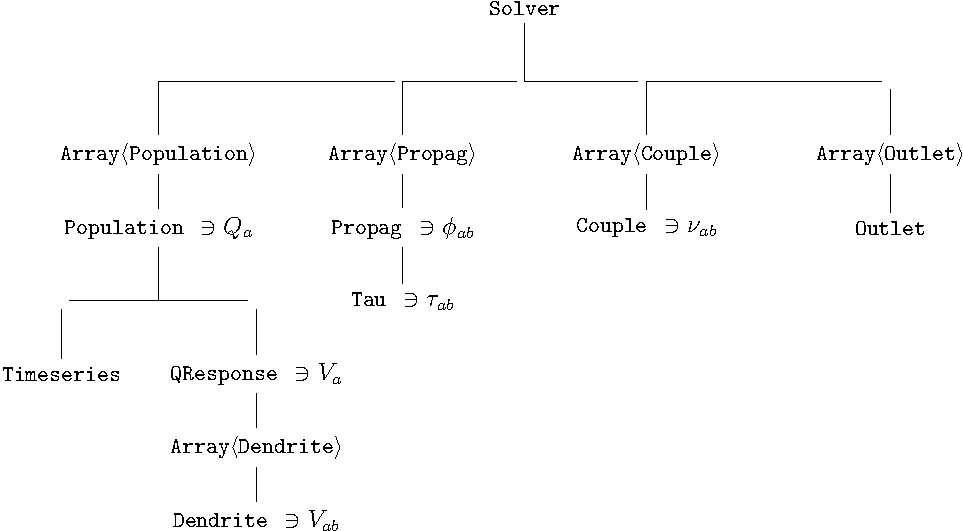
\includegraphics{class-hierarchy.pdf}
\caption{Schematic of the main class structures in \NF. Each line indicates that the bottom class is a member of the top class. The \type{a} $\ni b$ symbol indicates that the dynamical field $b(\mathbf{r},t)$ is a member of the class \type{a}. Inheritance structures are NOT illustrated.}
\label{fig:class}
\end{center}\end{figure}

\subsection{Class Array}
\label{sec:array}

\type{Array} is a container array to store objects that supports the \type{ofstream::<<} and \type{ifstream::>>} operators, as well as a \type{step(void)} function. This object typically is, but not necessarily has to be an \type{NF} object.

The \type{step(void)} function is equivalent to a \type{foreach(element).step()} in pseudocode. This function is encouraged over the use of \type{empty()}, \type{size()}, and \type{operator[]()}, which are discouraged to be used.

\subsection{Program flow}

Essentially, the program flow can be read from Fig.~\ref{fig:class}, so that objects take priority from top to bottom, left to right, both in terms of initialization and stepping through each timestep. A more detailed description is given below, and the reader is referred to the source code for complete description.

We use the semicolon to denote a succession of functions/procedures, and \type{a()} $\Rightarrow$ \type{b()} symbol to denote function \type{b()} as content of function \type{a()}.

\begin{center}
\begin{tabular}{ | l l p{11cm} | }
\hline \\

\type{main()}& $\Rightarrow$ &Initialize the config file, dump file and output file;\\[6pt]
&&\type{Solver::init()};\type{Solver::solve()};\\[6pt]
\type{Solver::init()}& $\Rightarrow$ &read in global parameters; Read in \type{CntMat};\\[6pt]
&&Construct \type{Population}; construct \type{Propag}; construct \type{Couple}; \type{Population::add2Dendrite()};\\[6pt]
&&Read configurations for \type{Population}, \type{Propag}, \type{Couple}, and \type{Output}.\\[6pt]
\type{Solver::solve()}& $\Rightarrow$ & \type{for(...) \{ Solver::step(); \type{Output::step()}; \} }\\[6pt]
\type{Solver::step()}& $\Rightarrow$ & \type{Population::step()}; \type{Propag::step()}; \type{Couple::step()};\\[6pt]
\type{Population::step()}& $\Rightarrow$ & \type{QResponse::step()} if neural population;\\[6pt]
&&\type{Timeseries::step()} if stimulus\\[6pt]
\type{QResponse::step()}& $\Rightarrow$ & \type{Dendrite::step()}; sum over \(V_{ab}\)

\\\hline
\end{tabular}
\end{center}

\subsection{Output routine}

To accommodate the coding interface for \type{NF::output}, the output routine of \NF involves 4 separate classes: \type{Outlet}, \type{Output}, \type{Outputs} and \type{Dumpf}.

\begin{tabular}{l p{16cm}}
	Class&Role\\
	\hline
	\type{Outlet}&Stores a reference to field variable (\type{vector<double>}) and its associated name.\\
	\type{Output}&Helper class in the parsing of which objects and which fields to output, according to the configuration file.\\
	\type{Outputs}&Contains \type{Array<Outlet>} and performs output routine.\\
	\type{Dumpf}&File handle (maybe to \type{stdout}) to output.
\end{tabular}

%\subsection{Other classes}

%\begin{description}
%\item[Modcouple] A class which provides synaptic coupling following a model proposed by Clearwater-Rennie for modelling neurotransmitter dynamics.
%\item[Random] Generates random numbers for Timeseries.
%\end{description}

\subsection{TODO}
\begin{enumerate}
\item check numerical entry of connection matrix
\end{enumerate}
\end{document}
